\documentclass[12pt]{article}

\usepackage{sbc-template}

\usepackage{graphicx,url}

%\usepackage[brazil]{babel}   
\usepackage[utf8]{inputenc}  
\usepackage[brazilian]{babel}
\usepackage[T1]{fontenc}     
\usepackage[opções]{subfigure}
\sloppy

\title{Instructions for Authors of SBC Conferences\\ Papers and Abstracts}

\author{Gustavo Belançon Mendes\inst{1}}


\address{Universidade Estadual de Maringá (UEM)\\
  Departamento de Informática\\
  Ciência da Computação
  \email{ra99037@uem.br}
}

\begin{document} 

\maketitle

\begin{resumo}
  A memória cache é uma memória que trabalha a uma velocidade mais elevada que as demais e que armazena os dados e as instruções mais utilizados pelo processador, facilitando o trabalho de busca de dados. Porém, quando a cache estiver totalmente ocupada, um dado recentemente utilizado irá encontrar dificuldades para ser gravado nela e seu acesso em outro instante teria que ser diretamente da memória principal, o que ocasionaria em um menor desempenho e um tempo maior de processamento. Para tentar evitar este problema, faz-se o uso de métodos de atualização da cache. Com base nisto, este trabalho realiza simulações, através do simulador Sniper, de dois tipos diferentes de algoritmos de atualização de cache, com o objetivo de analisar qual dos dois algoritmos apresentou um desempenho melhor na simulação da arquitetura do processador Xeon X5550 Gainestown. Como resultado, o algoritmo lru foi superior em 75\% dos testes.
\end{resumo}
     
\begin{abstract} 
  The cache memory is a memory that works with a higher speed than the others kind of memory, and it stores the data that was recently used by the processor, making it easier to the processor in fetching data. However, when the cache is full of data, a data recently used will find difficulties to be stored in cache and its access in other moment should be directly by the main memory, this fact would cause less performance and more time of processing. To try to avoid this situation, cache update policies are used. Based on this, this lab work realizes simulations, by the simulator Sniper, of two different types of algorithms of cache updates, that has the objective of analysis which of the two algorithms shows the best performance in the simulation of architecture of the Xeon X5550 Gainestown processor. As a result, the lru algorithm was better in 75\% of the tests.
\end{abstract}


\section{Introdução}

Conforme a tecnologia evolui, dispositivos tais como os computadores, servidores, aplicativos, entre outros, torna-se cada vez mais necessário para o usuário de tais tecnologias, uma capacidade maior de armazenamento e também uma velocidade maior, por parte destes dispositivos, para se processar os dados. 

A partir disso, surgiu um componente nas máquinas chamado memória cache, e que segundo \cite{brito:14}, nela contém uma cópia dos dados e instruções mais utilizadas recentemente. Trabalha juntamente com o processador e sua velocidade é superior à memória cache. Porém, se um dos dados ou instruções não foram processados a pouco tempo, como consequência, não estarão disponíveis na cache e ocorrerá o chamado cache \textit{miss}. Quando este último caso acontecer, o processador irá buscar o dado diretamente da memória principal, tal fato acaba gerando a desvantagem de ter um tempo maior de processamento, ao passo que o desempenho será menor.

Com isso, outro problema também surge, como saber qual dado deverá ser removido da cache para se armazenar aquele que foi recentemente lido. As políticas de atualização de cache são uma forma de corrigir o problema acima citado e realizar o gerenciamento do conteúdo armazenado na memória cache. 

Uma outra solução que pode auxiliar com os problemas de cache miss são as arquiteturas multiníveis, ou seja, ao invés de trabalhar com um único nível, pode ser integrado mais de um nível de cache para funcionarem simultaneamente, que segundo \cite{patterson:14}, o projeto para uma cache primária e secundária são significativamente diferentes porque a presença de outra muda a melhor escolha em comparação com uma de nível único. Os autores também ressaltam que uma estrutura de dois níveis permite que a cache primária se concentre em minimizar o tempo de acerto para produzir um ciclo de clock mais curto, enquanto permite que a cache secundária focalize a taxa de falhas no sentido de reduzir a penalidade dos longos tempos de acesso à memória.

Para este trabalho, foi apresentado a simulação de duas arquiteturas através do simulador Sniper, se baseando em configurações aproximadas às do processador Xeon X5550 Gainestown. Neste caso, o principal objetivo foi comparar o desempenho de dois diferentes algoritmos de atualização da cache.

\section{O Simulador Sniper}

O Sniper, segundo \cite{sniper:2019}, é um simulador de arquiteturas x86 paralelo, de alta velocidade e precisão. Este é capaz de simular um processador multi-core, baseado no modelo de intervalo de núcleo e possui também um suporte para visualização gráfica da simulação. Com isso o simulador fornece precisão e velocidade, com a possibilidade de alternar sua velocidade pela precisão de acordo com a necessidade de cada simulação, permitindo assim, a existência de um simulador flexível, explorando uma diversidade de opções de diferentes arquiteturas multi-núcleo, sejam elas homogêneas ou heterogêneas.

Este simulador permite a execução de simulações por tempo de programas multi-programados e multi-threads, aplicações de memória compartilhada executando de 10 até 100 ou mais núcleos, com uma velocidade alta se comparado com outros simuladores existentes. A principal característica do simulador é o seu modelo de núcleo, que é baseado em uma simulação dividida por intervalos, que faz deste modelo um mecanismo rápido. A simulação por intervalos aumenta o nível de abstração em uma simulação de arquitetura, que possibilita o desenvolvimento mais rápido por parte do simulador, isso se faz pulando um evento que teve miss como resultado, tal ação é chamada de intervalo. 

O simulador, e o seu modelo de núcleo utilizando intervalos, são úteis para estudos de nível de sistema e de núcleo que requerem mais detalhes que os modelos IPC, mas para os quais os simuladores de precisão de ciclo são muito lentos para permitir programas de grande tamanho a serem simulados. Outro benefício é que, o modelo de núcleo com intervalos permite a geração de pilhas de CPI, que mostram o número de ciclos perdidos devido a diferentes características do sistema, como a hierarquia de cache ou a previsão de desvio utilizada, levando a uma maior compreensão do efeito de cada componente na performance total do sistema.



\section{Arquitetura Simuladas}

As configurações das arquitetura simuladas neste laboratório, foram as mais próximas possíveis do padrão utilizado no processador Xeon X5550 Gainestown. Duas variações de configurações deste processador foram simuladas, entre uma e outra, apenas uma variável foi alterada, para podermos comparar diretamente as duas configurações. Para as duas configurações utilizamos as seguintes entradas: 

\begin{itemize}
    \item Clock: O clock é a frequência de número de ciclos por segundo com a qual o processador trabalha, ou seja, quantas ações ele consegue realizar em um determinado intervalo de tempo. No contexto deste laboratório, foi usado para as duas configurações o clock de 2.40 GHz;
    
    \item Previsão de desvio: É um método utilizado pelo processador para descobrir se o processador irá ou não executar uma instrução de desvio, as técnicas de previsão de desvio são importantes pois, segundo \cite{pizzol:05} as instruções de desvio provocam uma queda no desempenho dos processadores. Quando as previsões estiverem certas, tais desvios não causam interrupções. Para este laboratório foi considera a previsão de desvio pentium-m; 
    
    \item Algoritmo de atualização de cache: O objetivo principal das políticas de atualização de cache é gerenciar os dados presentes na cache e melhorar sua taxa de hit na cache. Os algoritmos de atualização de cache procuram diminuir as ocorrências de cache \textit{miss} e que o custo do cache \textit{miss} seja o mesmo para todos. Foram usados os seguintes algoritmos neste trabalho: lru e random;
    
    \item DRAM: Memória dinâmica de acesso aleatório ou \textit{Dynamic Random Access Memory}, este é um tipo de memória RAM que armazena cada bit de dados num capacitor, precisando que a informação seja atualizada o tempo todo para que permaneça armazenada. A configuração utilizada para a DRAM foi a \textit{constant}.
     
\end{itemize}

Portanto, como já citado, utilizaremos dois diferentes algoritmos de atualização de cache. Para o primeiro, a política lru(\textit{least recently used}), já para o segundo, foi usado o método \textit{random}.

\begin{itemize}

    \item Algoritmo lru: Utilização de uma pilha para armazenar em ordem o dados que acessaram mais recentemente a cache. Uma linha da cache é utilizada e inserida no topo da pilha, no base desta está o dados menos recentemente usado, este é removido para a inserção no topo do mais recente.

    \item Algoritmo random: Não utiliza nenhuma estrutura de dados, como fila, pilha, entre outros, para trabalhar. Escolhe aleatoriamente uma linha da cache a ser removida para a inserção de uma nova.

\end{itemize}

\section{Resultados e discussão}

A seguir foi descrito a metodologia que foi utilizada neste laboratório, assim como seu ambiente de instalação e as análises dos resultados obtidos através das simulações realizadas.

\subsection{Metodologia}
\begin{description}
\item[Software] Foi utilizado o simulador Sniper em sua versão 7.2, instalado e executado no sistema operacional Linux Ubuntu 18.04.
\item[Hardware] O simulador foi executado em uma máquina com as seguintes configurações: Processador Intel core i5 6200U (3 MB memória cache, 2 núcleos, 2.30GHz), 8GB RAM.
\item[Programas Simulados] Foram simulados 10 programas derivados do benchmark NPB-OMP 3.3.1, entre eles, BT, CG, DC, EP, FT, IS, LU, MG, SP, UA. Os significados de suas siglas são de acordo com o problema que solucionam. \textbf{BT} soluciona o problema \textit{"Block Tri-diagonal"}; \textbf{CG} Gradiente conjugado ou \textit{Conjugate Gradient}, acesso irregular de memória e comunicação; \textbf{DC} \textit{Data Cube}; \textbf{EP} \textit{Embarrassingly Parallel}; \textbf{FT} \textit{Discrete 3D fast Fourier Transform}, comunicação todos-para-todos; \textbf{LU} \textit{Lower-Upper Gauss-Seidel}; \textbf{MG} \textit{Multi-Grid} de uma sequência de malhas, comunicação de curta ou longa distância, memória intensiva; \textbf{SP} resolve \textit{Scalar Penta-diagonal}; \textbf{UA} \textit{Unstructured Adaptive mesh}, acesso dinâmico ou irregular à memória.

\item[Experimentos] Os programas citados acima, foram executados com duas configurações de arquitetura, que diferem apenas no algoritmo de atualização de cache. Portanto são duas simulações para cada programa, resultando em um total de 20 resultados diferentes, dois arquivos resultantes de cada programa, alternando sua política de atualização, lru e \textit{random}.

\item[Configurações da cache simulada] Nas simulações foram analisados dois algoritmos de atualização de cache, lru e \textit{random}. Para a cache L3, foi utilizado um tamanho total de 8 KB, e tamanho de bloco de 64 B, na cache L2 temos um espaço total de 512 KB e bloco de 64 B, já para a cache L1i e L1d, o armazenamento total é 32 KB e 64 B de tamanho de bloco para ambos.

\item[Avaliação] As taxas de cache miss e o total de cache miss serão avaliadas para concluir qual dos algoritmos de atualização de cache apresenta uma eficiência melhor, assim como o número de dados buscados na DRAM e dados de energia consumida na simulação de um programa. 

\item[Questões] Serão respondidas questões como: Qual é o melhor algoritmo de substituição de cache?, dos que foram simulados. Qual carregou mais dados da DRAM? Qual consumiu mais energia?.
\end{description}

\subsection{Resultados}

Todos os dados analisados desta seção foram obtidos através dos resultados da cache L1d, os programas foram todos simulados com a entrada W, bt.W.x, por exemplo. É apresentado a seguir, a análise dos resultados do total de cache miss, e a sua taxa em porcentagem. 

\begin{figure}[!h]
\centering
\subfigure[fig1a][Total de cache miss]{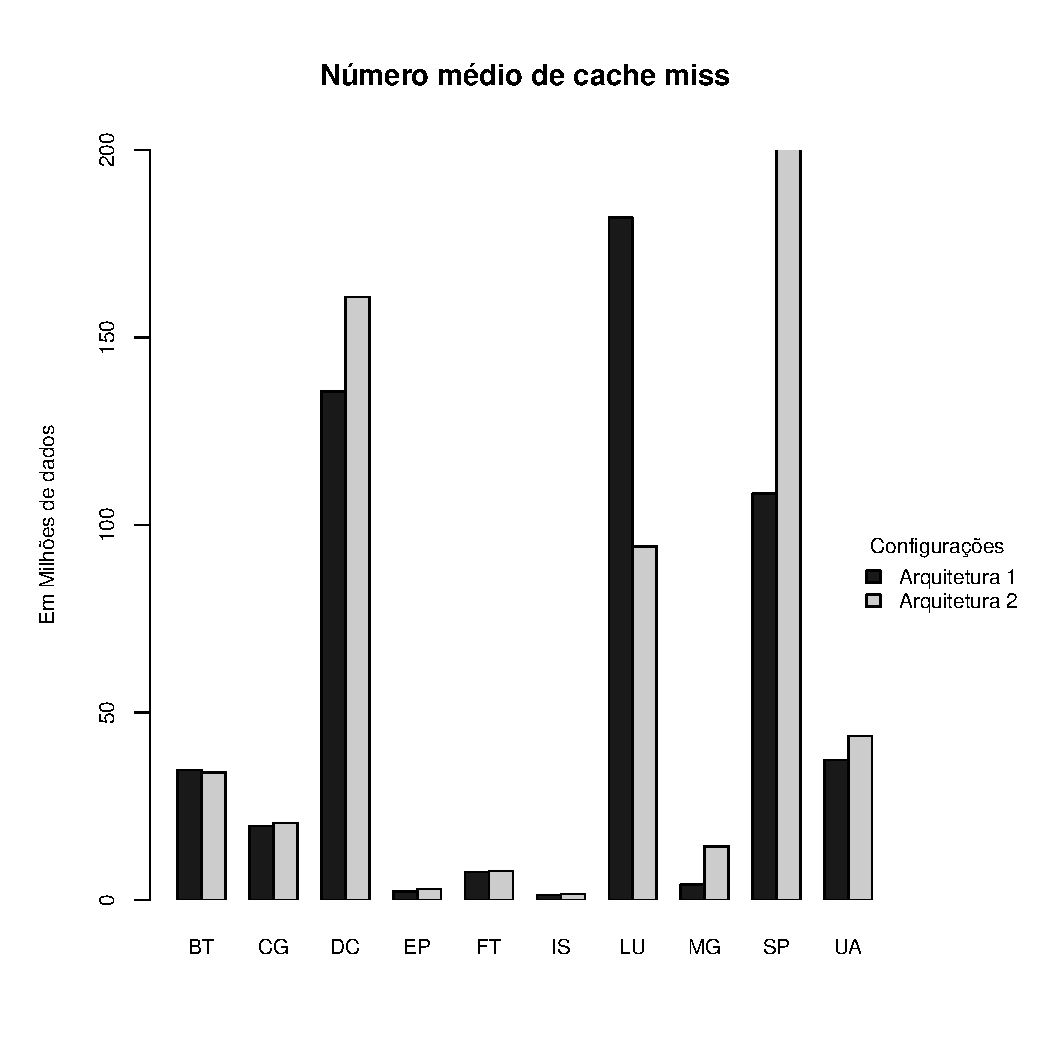
\includegraphics[width=.4\textwidth]{missCache.pdf}}
\subfigure[fig2b][Taxa miss em porcentagem]{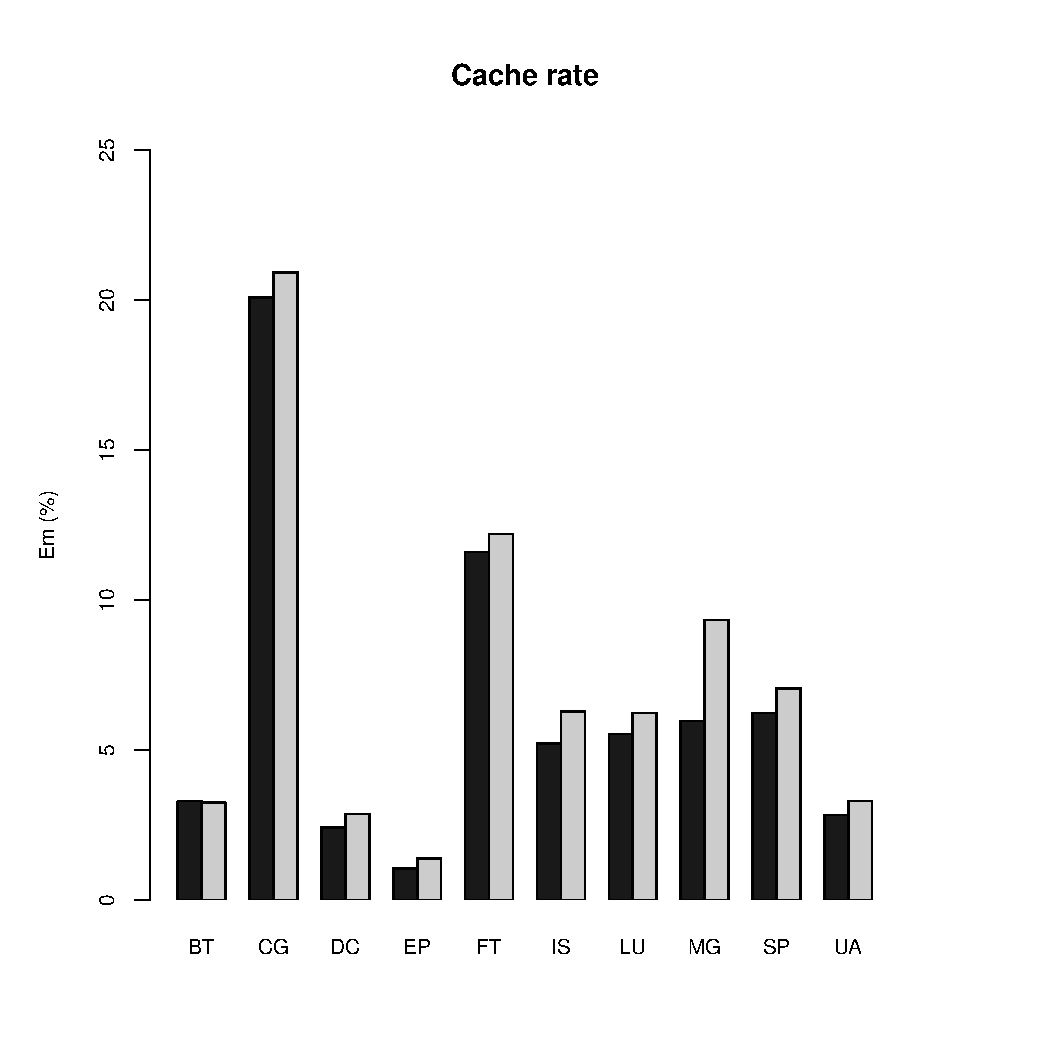
\includegraphics[width=.4\textwidth]{taxaMiss.pdf}}
\caption{Análise de cache miss dos programas}
\label{fig:fig1}
\end{figure}

Observando a Figura~\ref{fig:fig1}(a) o total de miss na cache, considerando uma média para os 8 cores simulados em cada programa, foi observado uma vantagem do algoritmo lru (Arquitetura 1 no gráfico) em relação ao \textit{random} (Arquitetura 2) na maioria dos casos. Em algumas simulações o \textit{random} se saiu melhor obtendo um número menor de cache miss, como foi com uma grande diferença no programa LU e em BT ligeiramente mais eficiente. 

Porém se observarmos a taxa de miss, que é o número total de acessos à cache dividido pelo número de miss, representada na Figura~\ref{fig:fig1}(b), temos que no programa LU o algoritmo lru se mostra com uma taxa de miss menor que \textit{random}, isso nos mostra que para a arquitetura 1 obter um número maior de cache miss, foi preciso acessar mais vezes a cache, enquanto que na política \textit{random} a cache foi acessada menos vezes, contudo apresentou uma taxa de miss maior, significando que a busca pelos dados diretamente da DRAM foi mais constante na segunda arquitetura do que na primeira, como exibido na Figura~\ref{fig:Fig2}. Concluimos a partir disso que, lru foi melhor que \textit{random} em nove dos dez casos.

\begin{figure}[!h]
\centering
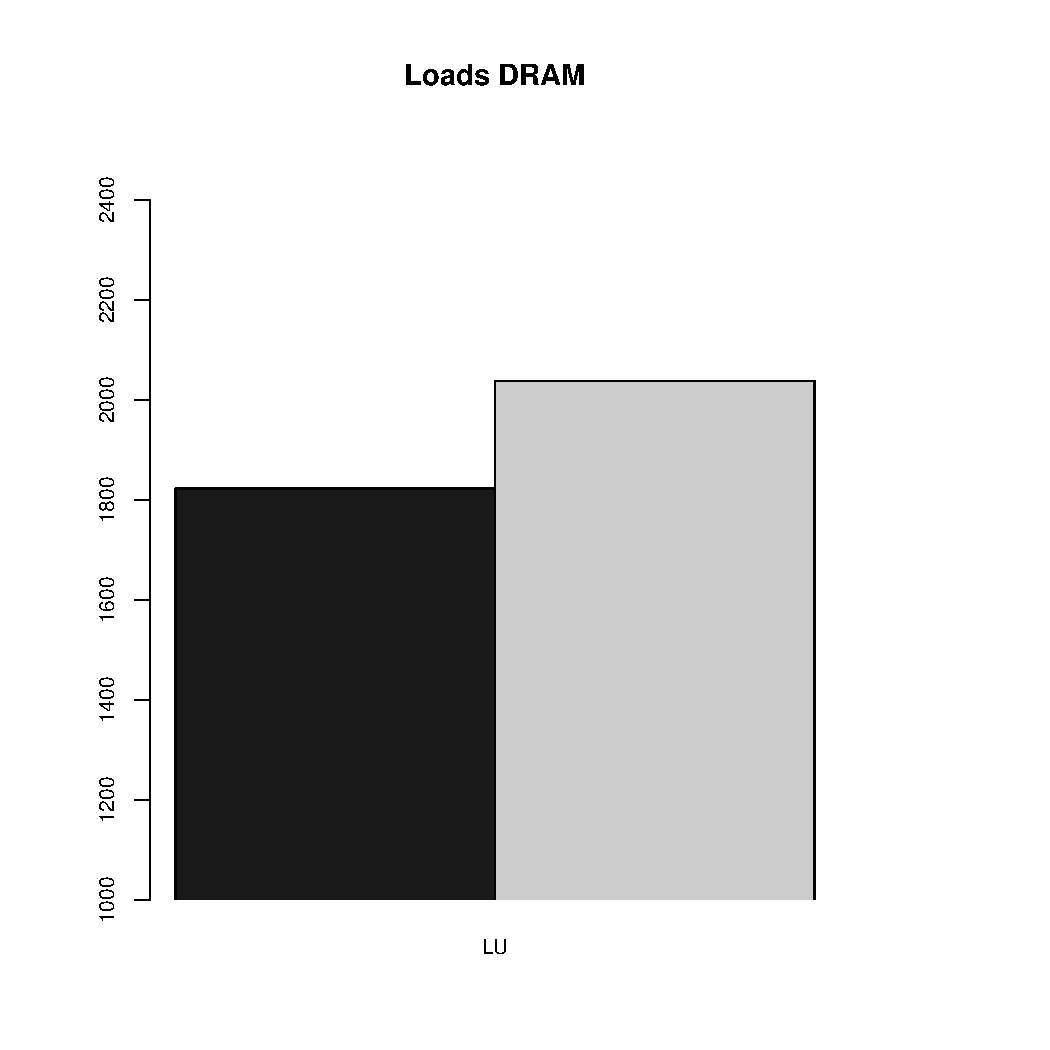
\includegraphics[width=.4\textwidth]{dramLoads.pdf}
\caption{Dados carregados da Dram, lru em preto e \textit{random} em branco}
\label{fig:Fig2}
\end{figure}

O gráfico a seguir mostra o consumo de energia de todos os programas executados, nele podemos concluir que o algoritmo lru possui um desempenho muito mais custoso no quesito energia, pois consumiu mais em oito dos dez casos de simulação, como visto na Figura~\ref{fig:Fig3}.

\begin{figure}[!h]
\centering
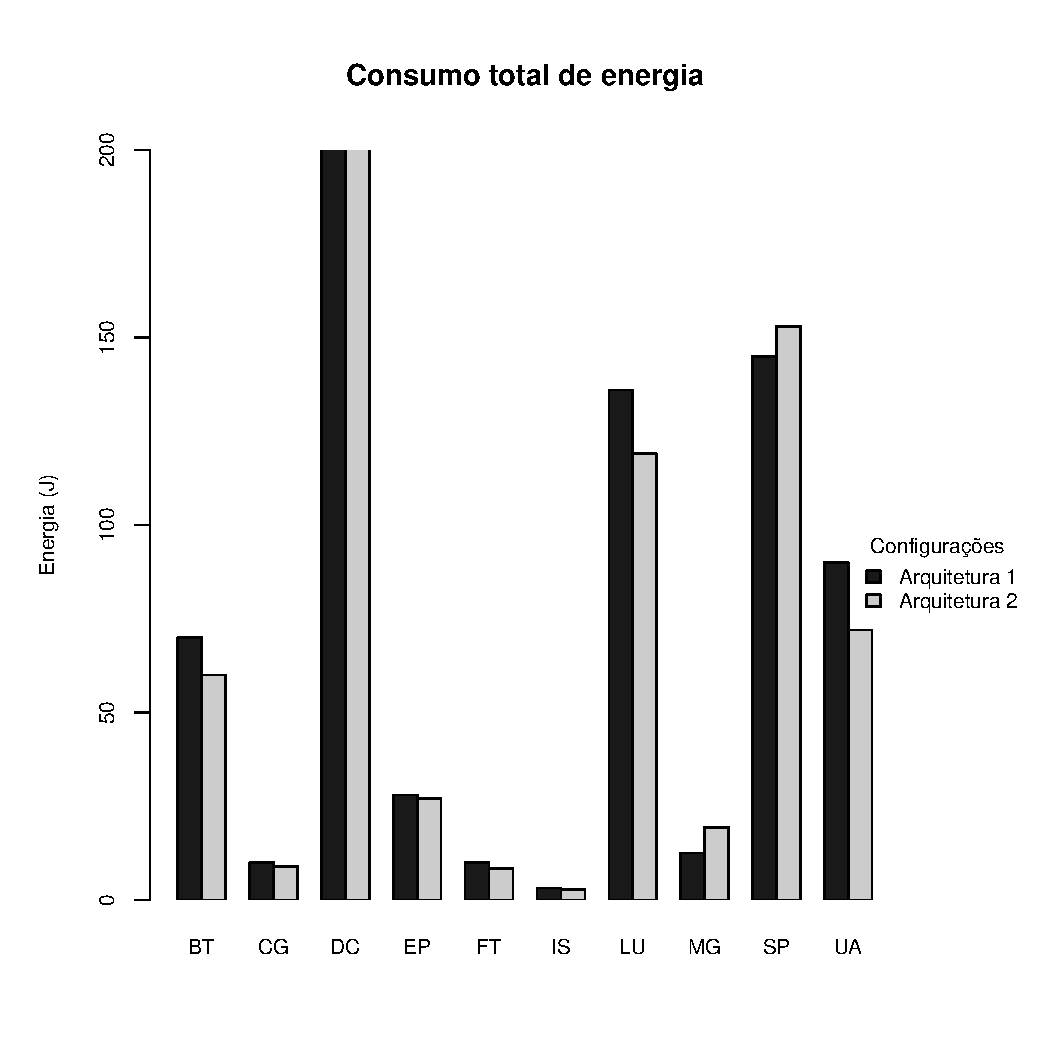
\includegraphics[width=.4\textwidth]{energia.pdf}
\caption{Energia consumida em Joules (J)}
\label{fig:Fig3}
\end{figure}

\section{Conclusão}

Os algoritmos de atualização de cache foram propostos para a intenção de manter uma forma de controlar os dados que estão armazenados na memória cache do processador, definem uma regra a ser seguida para substituir os dados. Atualmente, são vários os tipos de políticas de atualização disponíveis para serem implantadas com base em suas vantagens e desvantagens. Neste laborátorio, o objetivo foi avaliar os algoritmos lru e \textit{random}, executados para 10 diferentes programas.

Considerando os experimentos realizados, é possível concluir que os algoritmos de atualização possuem uma importante função no desempenho da memória cache. Como resultado, temos que o algoritmo lru possui um número menor de cache miss e uma taxa de miss menor que o \textit{random}, este resultado implica que o número de carregamentos de dados diretamente da DRAM foi menor para o lru em um dos casos que o número de miss foi maior também para o algoritmo lru, isso demonstra um desempenho melhor por parte dele. Por outro lado, o \textit{random} se mostrou mais eficiente em quase todos os programas na questão de gasto total de energia, que foi abaixo do lru. Logo, pode-se concluir que o algoritmo lru foi melhor que o \textit{random} em 75\% dos testes realizados.


\bibliographystyle{sbc}
\bibliography{sbc-template}

\end{document}
